\subsection{相贯线}
相贯线是两个立体相交,其表面所产生的交线。该交线是相交立体表面所共有的封闭线。
\subsubsection{两圆柱相交}
 \begin{figure}[htbp]
 \centering
\subfloat[]{\label{fig:xiangguan1}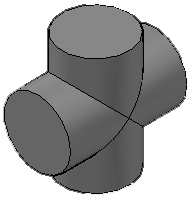
\includegraphics[scale=0.5]{xiangguan1.png}}\hspace{60pt}
\subfloat[]{\label{fig:xiangguan2}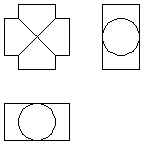
\includegraphics[scale=0.7]{xiangguan2.png}}
\caption{等径圆柱相交}
\end{figure}
图\ref{fig:xiangguan1}为两个直径相等的圆柱体相交。从图\ref{fig:xiangguan2}所示的三视图可知,相贯线的俯视图投影为上下重合的圆,左视图投影为左右重合的圆,主视图积聚为两条相交的直线。

 \begin{figure}[htbp]
 \centering
\subfloat[]{\label{fig:xiangguan3}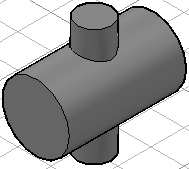
\includegraphics[scale=0.7]{xiangguan3.png}}\hspace{60pt}
\subfloat[]{\label{fig:xiangguan4}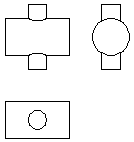
\includegraphics[scale=0.8]{xiangguan4.png}}
\caption{不等径圆柱相交}
\end{figure}
图\ref{fig:xiangguan3}为两个直径不相等的圆柱体相交。从图\ref{fig:xiangguan4}所示的三视图可知,相贯线的俯视图投影为上下重合的圆,主视图投影为前后重合的椭圆曲线,左视图左右重合的圆弧典线。

 \begin{figure}[htbp]
 \centering
\subfloat[]{\label{fig:xiangguan5}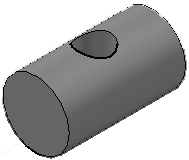
\includegraphics[scale=0.6]{xiangguan5.png}}\hspace{10pt}
\subfloat[]{\label{fig:xiangguan6}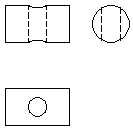
\includegraphics[scale=0.8]{xiangguan6.png}}\hspace{10pt}
\subfloat[]{\label{fig:xiangguan7}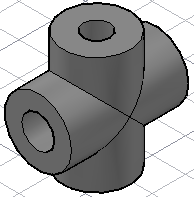
\includegraphics[scale=0.6]{xiangguan7.png}}\hspace{10pt}
\subfloat[]{\label{fig:xiangguan8}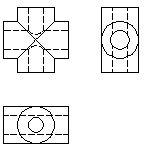
\includegraphics[scale=0.8]{xiangguan8.png}}
\caption{圆孔与圆柱相交和孔与孔相交}\label{fig:xiangguankong}
\end{figure}
图\ref{fig:xiangguankong}可知,孔与圆柱体的相贯线同圆柱体与圆相交的结果是基本一致的,只是其投影是不可见;孔与孔之间的相贯线也是如此。
\subsubsection{圆柱与平面体相交}
 \begin{figure}[htbp]
 \centering
\subfloat[]{\label{fig:xiangguan9}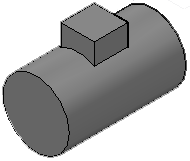
\includegraphics[scale=0.6]{xiangguan9.png}}\hspace{10pt}
\subfloat[]{\label{fig:xiangguan10}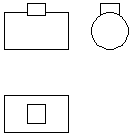
\includegraphics[scale=0.8]{xiangguan10.png}}\hspace{10pt}
\subfloat[]{\label{fig:xiangguan11}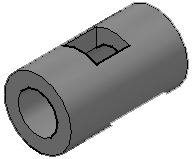
\includegraphics[scale=0.6]{xiangguan11.png}}\hspace{10pt}
\subfloat[]{\label{fig:xiangguan12}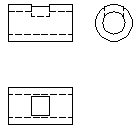
\includegraphics[scale=0.8]{xiangguan12.png}}
\caption{圆柱与平面体相交}\label{fig:xiangguannen}
\end{figure}
图\ref{fig:xiangguan9}为圆柱与长方体相交,图\ref{fig:xiangguan11}为圆筒与方孔相交,从两者的三视图可知,相贯线的俯视图投影为矩形,主视图投影为前后重合的直线,左视图为左右重合的圆弧。方孔与圆孔的相贯线不可见,结果如图\ref{fig:xiangguan12}所示。
\subsubsection{圆柱与圆锥相交}
 \begin{figure}[htbp]
 \centering
\subfloat[]{\label{fig:xiangguan13}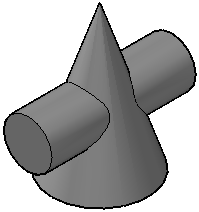
\includegraphics[scale=0.7]{xiangguan13.png}}\hspace{60pt}
\subfloat[]{\label{fig:xiangguan14}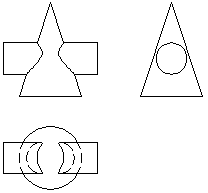
\includegraphics[scale=0.8]{xiangguan14.png}}
\caption{圆柱体与圆锥体相交}
\end{figure}
图\ref{fig:xiangguan13}为圆柱体与圆锥相交。从图\ref{fig:xiangguan14}所示的主视图可知,相贯线的主视图投影和前后重合的曲线,俯视图投影为由实线和虚线共同构成的封闭曲线,左视图投影为左右重合的圆。
\subsubsection{圆柱与球相交}
 \begin{figure}[htbp]
 \centering
\subfloat[]{\label{fig:xiangguan15}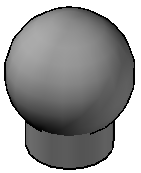
\includegraphics[scale=0.7]{xiangguan15.png}}\hspace{10pt}
\subfloat[]{\label{fig:xiangguan16}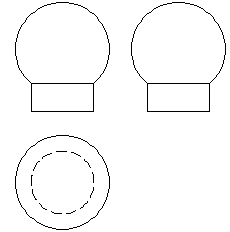
\includegraphics[scale=0.6]{xiangguan16.png}}\hspace{10pt}
\subfloat[]{\label{fig:xiangguan17}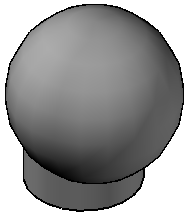
\includegraphics[scale=0.5]{xiangguan17.png}}\hspace{10pt}
\subfloat[]{\label{fig:xiangguan18}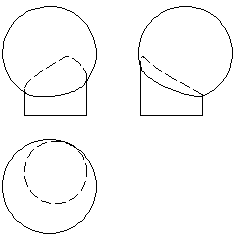
\includegraphics[scale=0.7]{xiangguan18.png}}
\caption{圆柱与平面体相交}\label{fig:xiangguanqiu}
\end{figure}
图\ref{fig:xiangguanqiu}为球与圆柱体相交的情况,当球心位于圆柱体轴线上时,相贯线为平面圆曲线;当球心不位于圆柱体轴线上时,相贯线为空间曲线。
\endinput